\section{Periodic Motion}

Name \rule{2.0in}{0.1pt}\hfill{}Section \rule{1.0in}{0.1pt}\hfill{}Date \rule{1.0in}{0.1pt}

{\bf Objectives }

To learn directly about some of the characteristics of periodic motion, 
namely period, frequency, and amplitude from the motion of a mass hanging from a spring. 
We will also investigate the relationships between position, velocity, acceleration, 
and force in simple harmonic motion.
Last, we will test the conservation of energy in simple harmonic motion.


\textbf{Apparatus} 

\begin{tabular}{p{2.5in}p{2.5in}}
$\bullet$  Spring                         & $\bullet$  Motion detector   \\[5pt]
$\bullet$  \textit{Pasco 750 Interface}   & $\bullet$  Force probe       \\[5pt]
$\bullet$  Variety of masses              & $\bullet$  \textit{DataStudio} software \\[5pt]
$\bullet$  2-meter stick                  &  \\[5pt]
\end{tabular}

%\begin{tabular}{|l|l|l|} \hline
%Two springs & Motion detector   & \textit{Science Workshop 750 Interface} \\ \hline
%Force probe & Variety of masses & \textit{DataStudio} software (Position and Velocity Graphs, SHM) \\ \hline
%\end{tabular}

\textbf{Introduction }

Periodic motion is motion that repeats itself. You can see the repetition in
the position-, velocity-, or acceleration-time graphs. The length of time to
go through one cycle and begin to repeat the motion is called the period $T$. The
number of cycles in each second is called the frequency $f$. The unit of frequency,
cycles per second, is given a special name --- Hertz.


\textbf{Activity  \stepcounter{activity}\arabic{activity}: Determination of the Spring Constant }

Measure the distance the spring stretches for five different masses and use
these data to determine the spring constant, $k$. 
Record your data and the result for $k$ in the space below.
\vspace{50mm}



\textbf{Activity  \stepcounter{activity}\arabic{activity}: Periodic Motion of a Mass-Spring System}

(a) Open the \textbf{Position \& Velocity Graphs} application in the \textbf{131 Workshop} submenu. 
Hang the large spring from the force probe hook with the
large diameter coils down and hang a 200-g mass from the spring. 
Place the motion detector facing up directly below the spring. 
Pull the mass straight downward about $7~ cm$, and let go.
Be careful to pull straight down so the motion of the weight is vertical and does not
swing sideways. 
Also be careful so the weight does not fall off the spring and strike the motion sensor.
Adjust the height of the support so that the mass comes no closer than $15~cm$ to the detector. 
Record data for a few seconds to display
position-time and velocity-time graphs of the motion. Sketch the graphs on the  axes below.

\textbf{Comment}: Note that when an object returns to the same position, it does not
necessarily mean that a cycle is ending. It must return to the same position,
and the velocity and acceleration must also return to the same values in both
magnitude and direction for this to be the start of a new cycle.

\vspace{0.3cm}
{\par\centering 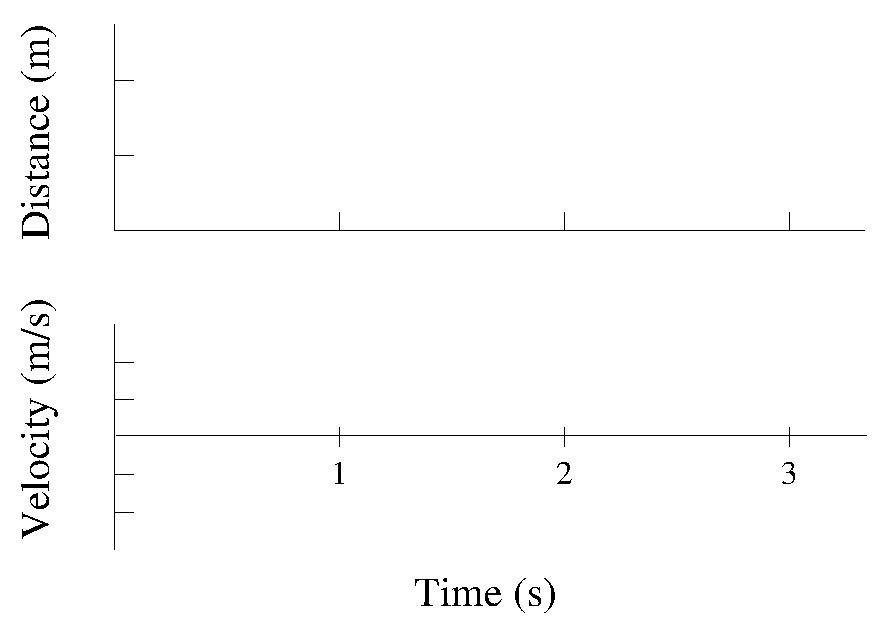
\includegraphics{periodic_motion/periodic_motion_fig1b.eps} \par}
\vspace{0.3cm}

(b) Label the graphs above with: ``B'' at the Beginning of a
cycle and ``E'' at the End of the same complete cycle, ``A''
on each spot where the mass is moving Away from the detector fastest, ``T''
on each spot where the mass is moving Toward the detector fastest, ``S''
on each spot where the mass is standing Still, ``F'' where the
mass is Farthest from the motion detector, and ``C'' where the mass
is Closest to the motion detector.

(c) Do the position and velocity graphs appear to have the same period? Do their
peaks occur at the same times? If not, how are the peaks related in time?
\vspace{20mm}

(d) Use the Smart Tool to measure the period and frequency of the motion. (For
better accuracy, measure the total time over as many cycles as possible and
divide by the number of cycles.)
\vspace{30mm}

(e) Using the Smart Tool, determine and record the maximum displacement
on your position graph. 
Next, collect data with the mass at rest hanging from the spring to find the equilibrium position. 
Subtract  this equilibrium \newpage value from the maximum displacement.
This is the amplitude of the motion.
Calculate and record here the amplitude of
the motion (the difference between the maximum displacement and the equilibrium
position).
\vspace{30mm}

\textbf{Simple Harmonic Motion }

The motion of a mass hanging from a spring that you looked at in Activity 2
is a close approximation to a kind of periodic motion called simple harmonic
motion (sometimes abbreviated SHM).

\textbf{Activity  \stepcounter{activity}\arabic{activity}: What Factors Determine the Period of the Mass-Spring System? }

(a) We now want to consider ways to change the period of the oscillator and make some predictions.
What will happen to the period if you increase the amplitude? 
\vspace{25mm}

(b) What will happen to the period if you increase the mass?
\vspace{25mm}


\textbf{Activity  \stepcounter{activity}\arabic{activity}: The Period of SHM and the Amplitude} 

(a) Repeat the procedure of Activity 2, but with a different starting position
of about 10 cm. (Warning: Do not make the amplitude so large that the mass
comes closer than 0.15 m from the motion detector.) When you have good graphs,
find and record the period and the amplitude using the methods described in
Activity 2. 
\vspace{20mm}

(b) Take ratios of the period and the amplitude of Activity 2 to those determined
here.
\vspace{20mm}

(c) Is there evidence that the period depends on amplitude? (Did the change
in amplitude result in a comparable change in period?) Explain. How does this
compare with your prediction?
\vspace{20mm}

\newpage

\textbf{Activity  \stepcounter{activity}\arabic{activity}: The Dependence of the Period of a SHM on the Mass} 

(a) Carefully measure the period for two other masses. Record the masses and
the measured periods in a table in the space below along with the mass and period from Activity 1.
\vspace{30mm}

(b) Does the period depend on the mass? Does it increase or decrease as mass
is increased?
\vspace{20mm}

\textbf{Comment:} You should have found that $T$ is independent of amplitude and increases with mass. 
The theoretical expression for the period is
\[T=2\pi \sqrt{\frac{m}{k}.}\]


\textbf{Velocity, Acceleration, Force and Energy }

In this investigation you will look more carefully at the distance, velocity
and acceleration graphs for simple harmonic motion. You will also look at the
force graph, and will examine the energy associated with simple harmonic motion.

\textbf{Activity  \stepcounter{activity}\arabic{activity}: Velocity, Acceleration, and Force for SHM} 

(a) Consider the motion you looked at in Activity 1 when the mass was 200 g
and the initial position was $5-10~ cm$. Sketch the position and velocity graphs
that you observed on the axes below using dashed lines.

\vspace{0.3cm}
{\par\centering 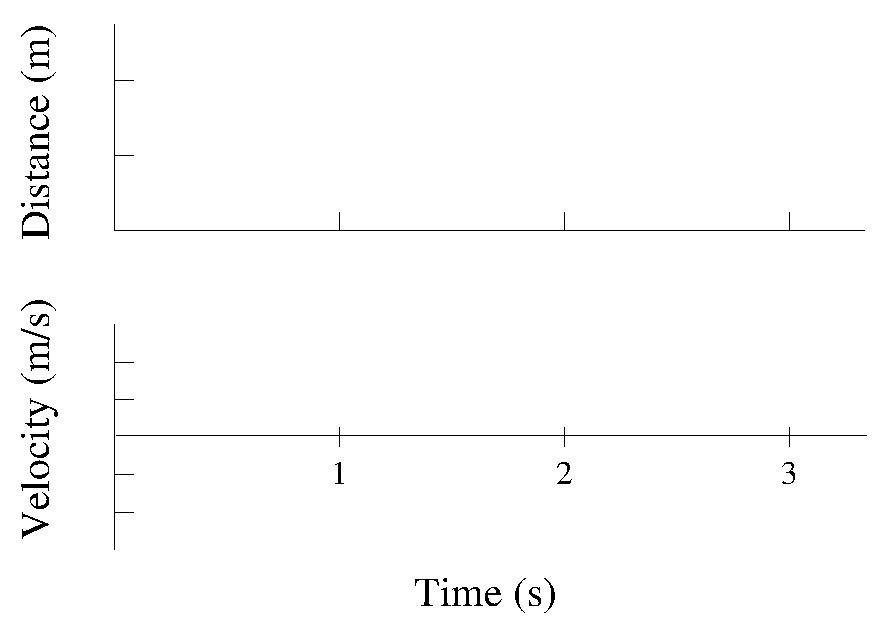
\includegraphics[width=4.0in]{periodic_motion/periodic_motion_fig1b.eps} \par}
\vspace{0.3cm}

\newpage

(b) Based on what you know about the relationships between velocity, acceleration,
and force, use dashed lines to sketch your predictions for the acceleration
and force graphs.

\vspace{0.3cm}
{\par\centering 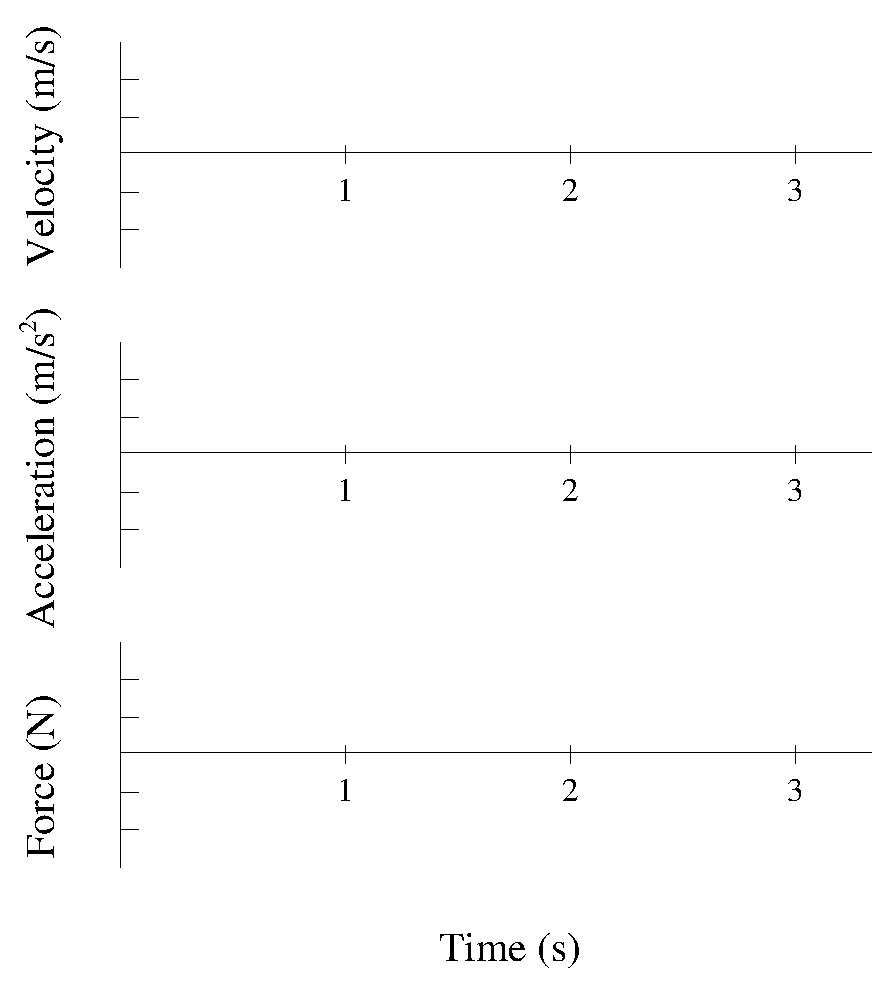
\includegraphics[width=4.0in]{periodic_motion/periodic_motion_fig3b.eps} \par}
\vspace{0.3cm}

(c) Suspend the 200-g mass from the spring and 
open the \textbf{SHM} application in the \textbf{131 Workshop} submenu. 
Start the mass oscillating with an amplitude of $5-10~ cm$ and record data for a few seconds.
When you have obtained good graphs, sketch the results on the above axes using
solid lines. Print your graph and attach to this unit.

(d) When the mass is at its maximum distance from the detector, is the velocity
maximum, minimum or some other value according to your graphs? Does this agree
with your predictions? Does this agree with your observations of the oscillating
mass? Explain.
\vspace{15mm}

(e) When the mass has its maximum positive velocity, is its distance from the
detector maximum, minimum, the equilibrium value or some other value according
to your graphs? What about when it reaches maximum negative velocity? Does this
agree with your predictions? Does this agree with your observations of the oscillating mass? Explain. 
\vspace{20mm}

\newpage

(f) According to your graphs, for what distances from the detector is the acceleration
maximum? For what distances is the acceleration zero? What is the velocity in
each of these cases?
\vspace{20mm}

(g) Compare the force and acceleration-time graphs. Describe any similarities.
Does the force graph agree with your prediction?
\vspace{20mm}

(h) From your graphs, what would you say is the relationship between force and
acceleration? 
\vspace{20mm}

(i) Compare the force and distance(position)-time graphs. What would you say
is the relationship between force and position? 
\vspace{20mm}

\textbf{Activity  \stepcounter{activity}\arabic{activity}: Energy of a Mass Undergoing SHM }

Now use the {\it DataStudio} graphs from the last activity to examine the energy relationships
in simple harmonic motion. 
To get the displacement from equilibrium you have to estimate the equilibrium position
on your position vs. time plot.
You can do this with the {\it SmartTool} by finding the point halfway between the 
minimum and maximum values of each 
oscillation.
The $x$ values must be determined relative to this equilibrium position (which represents a displacement of zero).
You will subtract this equilibrium value from the position measurement to get the displacement in
your analysis below.
Also, make sure the time axes for each graph are aligned.

(a) If we place the origin at the equilibrium point of the spring,
then where is the kinetic energy of the mass zero? Label these points
on your distance and velocity graphs above with a K.

(b) Calculate the elastic potential energy due to the spring at one of these
points. Label the point you use on your velocity and distance graphs with a
1. Use $U = {1\over 2}kx^{2}$, where 
$x$ is the distance from the equilibrium position
and $k$ is the force constant of the spring, 
which you have already measured in Activity 1. Use
the Smart Tool to measure $x$. Show your data and calculations in the space below. 
\vspace{20mm}

(c) Where is the potential energy zero? Label these points with a P
on your distance and velocity graphs.

(d) If you measured the kinetic energy at one of these points, what would you
expect its value to be? Explain.
\vspace{20mm}

\newpage

(e) Check your prediction. Calculate the kinetic energy at one of these points.
Label the point you use on your velocity graph with a 2. Use 
$K = {1\over 2} mv^{2}$.
Use the Smart Tool to determine $v$. Show your data and calculations in the space
below.
\vspace{20mm}

(f) Did your calculated kinetic energy agree with your prediction?
\vspace{20mm}

(g) If you calculated the potential and kinetic energies at a point where neither
of these was zero, what would you expect the total energy to be? Explain.
\vspace{20mm}

(h) Check your prediction. Make a table below (or make a spreadsheet and attach it to this unit)
with headings for $v~(m/s)$, position ($m$), $x~(m)$ where $x$ is the difference between the position
of the mass and the equilibrium position, $K$, $U$, and the total energy.
Pick at least six points where the mass has both kinetic and
potential energy, calculate them both ($K$ and $U$), and then calculate the total energy for each point ($K+U$). 
Label these points on your distance
and velocity graphs with numbers. 
Calculate the average and standard deviation of the total mechanical energy.
For information on calculating the average and
standard deviation, see \textbf{Appendix A}. Record the average and standard deviation here.
\vspace{60mm}

(i)  Is the total energy conserved?  Be quantitative in your answer.

